% Options for packages loaded elsewhere
\PassOptionsToPackage{unicode}{hyperref}
\PassOptionsToPackage{hyphens}{url}
\PassOptionsToPackage{dvipsnames,svgnames,x11names}{xcolor}
%
\documentclass[
  a4paper,
]{article}

\usepackage{amsmath,amssymb}
\usepackage{iftex}
\ifPDFTeX
  \usepackage[T1]{fontenc}
  \usepackage[utf8]{inputenc}
  \usepackage{textcomp} % provide euro and other symbols
\else % if luatex or xetex
  \usepackage{unicode-math}
  \defaultfontfeatures{Scale=MatchLowercase}
  \defaultfontfeatures[\rmfamily]{Ligatures=TeX,Scale=1}
\fi
\usepackage{lmodern}
\ifPDFTeX\else  
    % xetex/luatex font selection
\fi
% Use upquote if available, for straight quotes in verbatim environments
\IfFileExists{upquote.sty}{\usepackage{upquote}}{}
\IfFileExists{microtype.sty}{% use microtype if available
  \usepackage[]{microtype}
  \UseMicrotypeSet[protrusion]{basicmath} % disable protrusion for tt fonts
}{}
\makeatletter
\@ifundefined{KOMAClassName}{% if non-KOMA class
  \IfFileExists{parskip.sty}{%
    \usepackage{parskip}
  }{% else
    \setlength{\parindent}{0pt}
    \setlength{\parskip}{6pt plus 2pt minus 1pt}}
}{% if KOMA class
  \KOMAoptions{parskip=half}}
\makeatother
\usepackage{xcolor}
\usepackage[lmargin=2.54cm,rmargin=2.54cm,tmargin=2.54cm,bmargin=2.54cm]{geometry}
\setlength{\emergencystretch}{3em} % prevent overfull lines
\setcounter{secnumdepth}{3}
% Make \paragraph and \subparagraph free-standing
\ifx\paragraph\undefined\else
  \let\oldparagraph\paragraph
  \renewcommand{\paragraph}[1]{\oldparagraph{#1}\mbox{}}
\fi
\ifx\subparagraph\undefined\else
  \let\oldsubparagraph\subparagraph
  \renewcommand{\subparagraph}[1]{\oldsubparagraph{#1}\mbox{}}
\fi


\providecommand{\tightlist}{%
  \setlength{\itemsep}{0pt}\setlength{\parskip}{0pt}}\usepackage{longtable,booktabs,array}
\usepackage{calc} % for calculating minipage widths
% Correct order of tables after \paragraph or \subparagraph
\usepackage{etoolbox}
\makeatletter
\patchcmd\longtable{\par}{\if@noskipsec\mbox{}\fi\par}{}{}
\makeatother
% Allow footnotes in longtable head/foot
\IfFileExists{footnotehyper.sty}{\usepackage{footnotehyper}}{\usepackage{footnote}}
\makesavenoteenv{longtable}
\usepackage{graphicx}
\makeatletter
\def\maxwidth{\ifdim\Gin@nat@width>\linewidth\linewidth\else\Gin@nat@width\fi}
\def\maxheight{\ifdim\Gin@nat@height>\textheight\textheight\else\Gin@nat@height\fi}
\makeatother
% Scale images if necessary, so that they will not overflow the page
% margins by default, and it is still possible to overwrite the defaults
% using explicit options in \includegraphics[width, height, ...]{}
\setkeys{Gin}{width=\maxwidth,height=\maxheight,keepaspectratio}
% Set default figure placement to htbp
\makeatletter
\def\fps@figure{htbp}
\makeatother

\makeatletter
\makeatother
\makeatletter
\makeatother
\makeatletter
\@ifpackageloaded{caption}{}{\usepackage{caption}}
\AtBeginDocument{%
\ifdefined\contentsname
  \renewcommand*\contentsname{Table of contents}
\else
  \newcommand\contentsname{Table of contents}
\fi
\ifdefined\listfigurename
  \renewcommand*\listfigurename{List of Figures}
\else
  \newcommand\listfigurename{List of Figures}
\fi
\ifdefined\listtablename
  \renewcommand*\listtablename{List of Tables}
\else
  \newcommand\listtablename{List of Tables}
\fi
\ifdefined\figurename
  \renewcommand*\figurename{Figure}
\else
  \newcommand\figurename{Figure}
\fi
\ifdefined\tablename
  \renewcommand*\tablename{Table}
\else
  \newcommand\tablename{Table}
\fi
}
\@ifpackageloaded{float}{}{\usepackage{float}}
\floatstyle{ruled}
\@ifundefined{c@chapter}{\newfloat{codelisting}{h}{lop}}{\newfloat{codelisting}{h}{lop}[chapter]}
\floatname{codelisting}{Listing}
\newcommand*\listoflistings{\listof{codelisting}{List of Listings}}
\makeatother
\makeatletter
\@ifpackageloaded{caption}{}{\usepackage{caption}}
\@ifpackageloaded{subcaption}{}{\usepackage{subcaption}}
\makeatother
\makeatletter
\@ifpackageloaded{tcolorbox}{}{\usepackage[skins,breakable]{tcolorbox}}
\makeatother
\makeatletter
\@ifundefined{shadecolor}{\definecolor{shadecolor}{rgb}{.97, .97, .97}}
\makeatother
\makeatletter
\makeatother
\makeatletter
\makeatother
\ifLuaTeX
  \usepackage{selnolig}  % disable illegal ligatures
\fi
\usepackage[]{biblatex}
\addbibresource{../../../../references.bib}
\IfFileExists{bookmark.sty}{\usepackage{bookmark}}{\usepackage{hyperref}}
\IfFileExists{xurl.sty}{\usepackage{xurl}}{} % add URL line breaks if available
\urlstyle{same} % disable monospaced font for URLs
\hypersetup{
  pdftitle={La Economía Peruana de 1970 a 1990 Un Análisis de sus Períodos y Desafíos},
  pdfauthor={Achalma Mendoza Elmer Edison},
  colorlinks=true,
  linkcolor={blue},
  filecolor={Maroon},
  citecolor={Blue},
  urlcolor={Blue},
  pdfcreator={LaTeX via pandoc}}

\title{La Economía Peruana de 1970 a 1990 Un Análisis de sus Períodos y
Desafíos}
\usepackage{etoolbox}
\makeatletter
\providecommand{\subtitle}[1]{% add subtitle to \maketitle
  \apptocmd{\@title}{\par {\large #1 \par}}{}{}
}
\makeatother
\subtitle{Una revisión detallada de los gobiernos y políticas económicas
que marcaron la evolución del Perú.}
\author{Achalma Mendoza Elmer Edison}
\date{2023-06-03}

\begin{document}
\maketitle
\ifdefined\Shaded\renewenvironment{Shaded}{\begin{tcolorbox}[borderline west={3pt}{0pt}{shadecolor}, interior hidden, boxrule=0pt, enhanced, breakable, frame hidden, sharp corners]}{\end{tcolorbox}}\fi

\renewcommand*\contentsname{Contenidos}
{
\hypersetup{linkcolor=}
\setcounter{tocdepth}{3}
\tableofcontents
}
\hypertarget{quuxe9-es-el-cambio-climuxe1tico-y-cuxf3mo-afecta-a-nuestras-vidas}{%
\section{¿Qué es el cambio climático y cómo afecta a nuestras
vidas?}\label{quuxe9-es-el-cambio-climuxe1tico-y-cuxf3mo-afecta-a-nuestras-vidas}}

El cambio climático se refiere a la alteración del clima atribuida a
causas naturales y, de manera directa o indirecta, a la actividad
humana. Provoca cambios en la composición de la atmósfera a nivel global
y se suma a la variabilidad natural del clima a lo largo del tiempo,
afectando diversos parámetros climáticos como la temperatura, las
precipitaciones y la nubosidad, entre otros. Cuando el cambio climático
amenaza gravemente a las sociedades, las economías y la naturaleza, se
convierte en un problema peligroso.

El impacto del cambio climático se extiende a todas las personas. Sus
consecuencias potenciales son enormes, incluyendo la escasez de agua
potable, cambios significativos en las condiciones de producción de
alimentos y un aumento en la mortalidad debido a eventos extremos como
inundaciones, tormentas, sequías y olas de calor. Es importante destacar
que el cambio climático no es solo un fenómeno ambiental, sino que
también tiene profundas implicaciones económicas y sociales. Los países
más pobres, que suelen estar menos preparados para hacer frente a
cambios rápidos, serán los más afectados por las graves consecuencias.

Además, se prevé la extinción de numerosas especies de animales y
plantas, ya que los hábitats están cambiando a una velocidad tan rápida
que muchas especies no pueden adaptarse a tiempo. La Organización
Mundial de la Salud ha advertido sobre las amenazas para la salud de
millones de personas debido al aumento de enfermedades como la malaria,
la desnutrición y las enfermedades transmitidas por el agua. En el caso
de Perú, su ubicación geográfica y sus características socioeconómicas
lo hacen particularmente vulnerable al cambio climático.

Aquí está el texto mejorado:

\hypertarget{cuxf3mo-mitigar-el-cambio-climuxe1tico}{%
\section{¿Cómo mitigar el cambio
climático?}\label{cuxf3mo-mitigar-el-cambio-climuxe1tico}}

La lucha contra el cambio climático es un desafío importante, pero con
el esfuerzo colectivo y la implementación de medidas adecuadas de
mitigación, podemos reducir al mínimo los daños. Para lograrlo, es
necesario tomar las siguientes acciones:

\begin{itemize}
\item
  Mejorar la eficiencia energética y dar prioridad a las fuentes de
  energía renovable en lugar de depender de los combustibles fósiles.
\item
  Fomentar el uso del transporte público y promover la movilidad
  sostenible, alentando el uso de la bicicleta para desplazamientos
  urbanos, reduciendo los vuelos en avión y favoreciendo los viajes en
  tren y en coche compartido.
\item
  Impulsar la adopción de prácticas ecológicas en la industria, la
  agricultura, la pesca y la ganadería, promoviendo la sostenibilidad
  alimentaria, el consumo responsable y la aplicación de la regla de las
  3R (reducir, reutilizar y reciclar).
\item
  Imponer impuestos al uso de combustibles fósiles y establecer mercados
  de emisiones de CO2, con el objetivo de desincentivar su utilización y
  promover la reducción de las emisiones de gases de efecto invernadero.
\end{itemize}

Además, es fundamental promover la conciencia ambiental y la educación
sobre el cambio climático en todos los niveles de la sociedad, así como
fomentar la colaboración internacional para abordar este desafío global
de manera efectiva. Juntos, podemos marcar la diferencia en la
mitigación del cambio climático y construir un futuro más sostenible.

\hypertarget{cuxf3mo-adaptarnos-a-los-cambios}{%
\section{¿Cómo adaptarnos a los
cambios?}\label{cuxf3mo-adaptarnos-a-los-cambios}}

Cuando se trata de adaptarnos a las consecuencias del cambio climático,
existen diversas medidas que nos ayudan a reducir nuestra
vulnerabilidad. A continuación, se presentan algunas acciones clave:

\begin{itemize}
\item
  Construir edificaciones e infraestructuras más seguras y sostenibles,
  teniendo en cuenta los posibles impactos del cambio climático. Además,
  es importante enfocarse en la restauración de los ecosistemas dañados,
  lo que contribuye a fortalecer la resiliencia frente a eventos
  climáticos extremos.
\item
  Llevar a cabo la restauración paisajística y la reforestación de
  bosques, ya que estas acciones no solo promueven la conservación de la
  biodiversidad, sino que también ayudan a mitigar los efectos del
  cambio climático.
\item
  Fomentar la diversificación de los cultivos, de manera que sean
  capaces de adaptarse a las condiciones climáticas cambiantes. Esto
  implica explorar variedades de cultivos más resistentes y promover
  prácticas agrícolas sostenibles que se adapten a los cambios en los
  patrones de lluvia y temperatura.
\item
  Promover la investigación y el desarrollo de soluciones innovadoras
  para la prevención y gestión de catástrofes naturales, con el objetivo
  de anticiparse y responder de manera eficiente a los eventos
  climáticos extremos.
\item
  Establecer protocolos de actuación claros y eficaces para situaciones
  de emergencia climática, con el fin de minimizar los riesgos y
  proteger a la población de manera rápida y efectiva.
\end{itemize}

\hypertarget{cuxf3mo-promover-reformas-inclusivas}{%
\subsection{¿Cómo promover reformas
inclusivas?}\label{cuxf3mo-promover-reformas-inclusivas}}

Una forma efectiva de promover reformas inclusivas es a través de la
``Creación y Fomento de Capacidades''. Este enfoque se basa en difundir
y concienciar a la ciudadanía sobre los problemas ambientales,
especialmente aquellos relacionados con el cambio climático, al mismo
tiempo que se fomenta la educación, la sensibilización y la
investigación sobre este tema en Perú.

La creación y el fomento de capacidades se refieren a fortalecer el
conocimiento y las habilidades de las personas, permitiéndoles
participar de manera activa y significativa en la toma de decisiones y
acciones relacionadas con el cambio climático. Algunas acciones clave en
este enfoque incluyen:

\begin{itemize}
\item
  Promover programas educativos y de sensibilización sobre el cambio
  climático, dirigidos a diferentes grupos de la sociedad, desde
  estudiantes hasta profesionales y líderes comunitarios. Estos
  programas deben abordar tanto los aspectos científicos como los
  sociales y económicos del cambio climático, fomentando una comprensión
  integral del tema.
\item
  Impulsar la investigación y el desarrollo de soluciones innovadoras
  para abordar los desafíos del cambio climático. Esto incluye apoyar la
  investigación científica, tecnológica y social, así como fomentar la
  colaboración entre instituciones académicas, organizaciones de la
  sociedad civil y el sector privado.
\item
  Facilitar el acceso a recursos y oportunidades para que las
  comunidades vulnerables puedan adaptarse y mitigar los impactos del
  cambio climático. Esto implica brindar apoyo técnico, financiero y de
  capacitación para promover la resiliencia en estas comunidades.
\item
  Fomentar la participación activa de la sociedad civil en la toma de
  decisiones y en la formulación de políticas relacionadas con el cambio
  climático. Esto incluye la creación de espacios de diálogo y consulta,
  así como la promoción de la inclusión de diferentes grupos de interés
  en el proceso de toma de decisiones.
\end{itemize}

Aquí está el texto mejorado:

\hypertarget{otros-problemas-ambientales.}{%
\section{Otros problemas
ambientales.}\label{otros-problemas-ambientales.}}

\begin{enumerate}
\def\labelenumi{\alph{enumi}.}
\tightlist
\item
  El cambio climático no es el único factor que amenaza el desarrollo
  sostenible. Existen otros componentes críticos del capital natural que
  también están en peligro, como la pérdida de biodiversidad, la
  contaminación del aire, el uso insostenible del agua, la erosión del
  suelo y la deforestación.
\end{enumerate}

Utilizando la afirmación anterior, planteamos un modelo económico y un
modelo econométrico que especifica las variables y los datos que se
utilizarían para analizar estas variables.

Ante los desafíos del cambio climático y las amenazas a nuestro capital
natural, se propone el uso de un modelo económico que busca
contrarrestar estos efectos:

\textbf{Modelo de Economía Circular}

El modelo de economía circular surge como una alternativa al tradicional
modelo económico de desperdicio y extracción, que contribuye al cambio
climático.

El modelo de economía circular ofrece un marco de soluciones sistémicas
para el desarrollo económico, abordando de manera integral el cambio
climático, la pérdida de biodiversidad, el incremento de residuos y la
contaminación. Además, este modelo se basa en el diseño y el uso de
energías y materiales renovables, revolucionando la forma en que
diseñamos, producimos y consumimos. Se fundamenta en tres principios
clave: eliminar residuos y contaminación, mantener productos y
materiales en uso, y regenerar sistemas naturales (Albaladejo \& Mirazo,
2021).

En este sentido, se plantean las variables con las que se desarrollará
el modelo económico circular y se definen sus respectivos indicadores:

\begin{itemize}
\tightlist
\item
  \textbf{Variable endógena:} Desarrollo sostenible
\item
  \textbf{Variables exógenas:} Pérdida de biodiversidad, contaminación
  del aire, uso insostenible del agua y deforestación.
\end{itemize}

A continuación, se proporciona la definición conceptual, los indicadores
y las unidades de medida de estas variables:

\textbf{Tabla 1}

\emph{Variables e indicadores del modelo de economía circular}

\begin{longtable}[]{@{}
  >{\raggedright\arraybackslash}p{(\columnwidth - 4\tabcolsep) * \real{0.3333}}
  >{\raggedright\arraybackslash}p{(\columnwidth - 4\tabcolsep) * \real{0.3333}}
  >{\raggedright\arraybackslash}p{(\columnwidth - 4\tabcolsep) * \real{0.3333}}@{}}
\toprule\noalign{}
\begin{minipage}[b]{\linewidth}\raggedright
Variable
\end{minipage} & \begin{minipage}[b]{\linewidth}\raggedright
Definición Conceptual
\end{minipage} & \begin{minipage}[b]{\linewidth}\raggedright
Indicador
\end{minipage} \\
\midrule\noalign{}
\endhead
\bottomrule\noalign{}
\endlastfoot
\textbf{Variable Endógena:} Desarrollo sostenible & Se refiere al
desarrollo que satisface las necesidades del presente sin comprometer la
capacidad de las futuras generaciones, garantizando el equilibrio entre
crecimiento económico, cuidado del medio ambiente y bienestar social. &
Índice de Enriquecimiento inclusivo (PBI verde) \\
\textbf{Variables Exógenas:} & & \\
Contaminación del aire & Se refiere a la presencia en el aire de
partículas pequeñas o productos gaseosos secundarios que pueden
representar riesgos, daños o molestias para las personas, las plantas y
los animales expuestos a dicho ambiente. & Emisiones anuales de CO2 en
toneladas por año \\
Pérdida de biodiversidad & Hace referencia a la disminución o
desaparición de los seres vivos que habitan el planeta, incluyendo los
distintos niveles de organización biológica y su variabilidad genética,
así como los patrones naturales presentes en los ecosistemas. & Número
de especies de fauna y flora \\
Deforestación & Se refiere a la eliminación completa de un bosque
mediante la tala, para dar espacio a otros usos en su lugar. & Pérdida
de superficie forestal medida en hectáreas \\
\end{longtable}

En base a lo expuesto, planteamos el siguiente modelo econométrico:

\[ PBI_{V} = \beta_{0} + \beta_{1}CA + \beta_{2}BIO + \beta_{3}DEF + \mu \]

Donde:

PBI\_\{V\}: Producto Bruto Interno Verde

CA: Contaminación del aire

BIO: Pérdida de biodiversidad

DEF: Deforestación

μ: Término de perturbación

Con este modelo, buscamos analizar la relación entre el Producto Bruto
Interno Verde y las variables exógenas de contaminación del aire,
pérdida de biodiversidad y deforestación. Estos datos nos permitirán
comprender cómo influyen estos factores en el desarrollo sostenible y
orientar las políticas y acciones necesarias para promover un
crecimiento económico más sostenible y resiliente al cambio climático.

\begin{enumerate}
\def\labelenumi{\alph{enumi}.}
\setcounter{enumi}{1}
\tightlist
\item
  Las prácticas agrícolas insostenibles tienen un impacto negativo en el
  medio ambiente, erosionando el suelo, agotando las reservas de agua
  dulce y reduciendo la superficie forestal. Estas acciones provocan la
  disminución de la capacidad del planeta para absorber dióxido de
  carbono y contribuyen a la pérdida de biodiversidad, la cual es
  fundamental para adaptarse al cambio climático.
\end{enumerate}

Utilice la afirmación (b) y explique y grafique la relación entre las
prácticas agrícolas insostenibles y la pérdida de biodiversidad.

Para comprender la relación entre las prácticas agrícolas insostenibles
y la pérdida de biodiversidad, podemos analizarla tanto de manera
explicativa como visual. En la figura 1, presentada a continuación, se
grafica esta relación:

\begin{figure}

\caption{Figura 1: Relación entre las prácticas agrícolas insostenibles
y la pérdida de biodiversidad}

{\centering 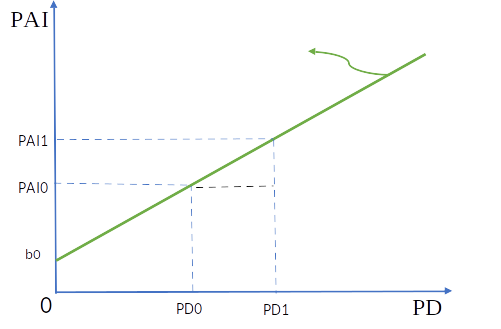
\includegraphics{20230603001915.png}

}

\end{figure}

En la gráfica, se observa una relación positiva entre las prácticas
agrícolas insostenibles (PAI) y la pérdida de diversidad (PD). A medida
que las prácticas agrícolas insostenibles aumentan, la pérdida de
biodiversidad también se incrementa. Sin embargo, la magnitud del
impacto de las prácticas agrícolas insostenibles en la pérdida de
biodiversidad se mide mediante la sensibilidad o elasticidad, que se
calcula como el cambio porcentual de las prácticas agrícolas
insostenibles dividido por el cambio porcentual en la pérdida de
diversidad.

La ecuación que representa esta relación es:

PD = b0 + b1 * PAI

↑PAI → ↑PD:

A mayor cantidad de prácticas agrícolas insostenibles, se genera una
mayor pérdida de diversidad.

Donde b1 es la sensibilidad y mide la variación de la pérdida de
biodiversidad ante cambios en las prácticas agrícolas insostenibles.

Este análisis se fundamenta en el respaldo teórico proporcionado por la
Secretaría del Convenio sobre la Diversidad Biológica (2008), que señala
cómo en las últimas cinco décadas la expansión agrícola, especialmente
en zonas tropicales y subtropicales, ha reducido significativamente los
niveles de diversidad biológica y los servicios ecosistémicos en áreas
clave, socavando así la sostenibilidad a largo plazo de la producción
agrícola en sí (p.~22).

\hypertarget{el-peruxfa-es-vulnerable-al-cambio-climuxe1tico}{%
\subsection{El Perú es vulnerable al cambio
climático}\label{el-peruxfa-es-vulnerable-al-cambio-climuxe1tico}}


\printbibliography


\end{document}
